\chapter{Aplicação}
\label{c.aplicacao}

\section{Descrição da Aplicação}
\label{s.descricao}

Na aplicação a ser desenvolvida, o usuário irá explorar uma área que conterá vários objetos. O objetivo do usuário será de se movimentar no espaço através de um controle físico, procurar objetos específicos ao redor movimentando a cabeça e executar ações sobre os mesmos.

A fim de contextualizar o usuário no ambiente e definir os objetos que receberão ações, a aplicação terá como tema o mosquito Aedes aegypti, onde o usuário terá que eliminar os focos do mosquito no quintal de uma casa. 

O \citeonline{riodejaneiro} publicou em seu website os lugares propícios para a reprodução do mosquito juntamente com as precauções que as pessoas devem tomar para a eliminação do Aedes aegypti. Os usuários da aplicação deverão realizar seis das quinze providências fornecidas pelo website que são:

•	Coloque areia no prato dos vasos de plantas.

•	Mantenha o saco de lixo bem fechado e fora do alcance de animais até o recolhimento pelo serviço de limpeza urbana. Não jogue lixo em terrenos baldios.

•	Troque diariamente a água dos bebedouros de animais e aves e limpe-os com escova ou bucha.

•	Entregue seus pneus velhos ao serviço de limpeza urbana ou guarde-os sem água em local coberto e abrigados da chuva.

•	Guarde as garrafas vazias sempre de cabeça para baixo e de preferência em local coberto.

•	Limpe constantemente as calhas, remova tudo que possa impedir a passagem da água, a laje e a piscina de sua casa

\section{Ações}
\label{s.acoes}

O usuário contará com cinco ações dentro da aplicação: andar, agachar, focar, selecionar e abrir o menu. Os caminhos possíveis que o usuário poderá percorrer serão determinados por objetos que servirão como guias dentro da aplicação. Ao selecionar os guias, o usuário irá caminhar até os mesmos, podendo atingir seis posições no cenário como mostra a Figura X.

\begin{figure}[h]
	\caption{\small Posições possíveis na aplicação}
	\centering
	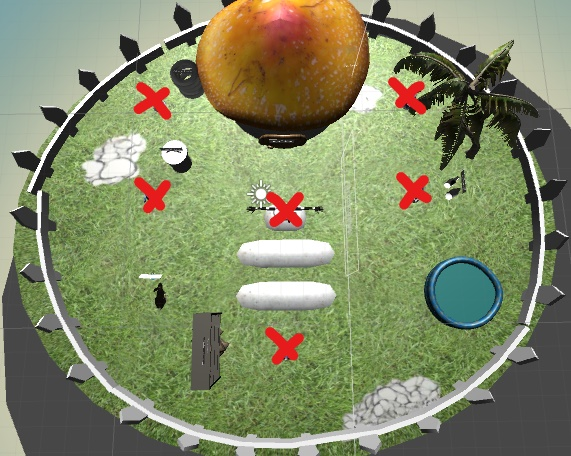
\includegraphics[scale=0.50]{Imagens/posicoes.jpg}
	\label{f.posicoes}
	\legend{\small Fonte: Elaborada pelo autor.}
\end{figure}

Os objetos que poderão sofrer ações possuem um menu que é acionado enquanto o usuário foca o objeto. Este menu mostrará qual ação é permitida para aquele determinado objeto e o usuário poderá executar a ação ao selecionar o menu. A tabela X demonstra como cada controle executará as ações citadas acima. 


\begin{longtable}{p{2.2cm}|p{2.2cm}|p{2.2cm}|p{2.2cm}|p{2.2cm}|p{2.2cm}}
	\caption[]{Ações dos dispositivos}  \\
	\label{t.acoes}
	\textbf{\small Dispositivo de controle} & \multicolumn{5}{c}{\textbf{\small Ações}}  \\ \hline \hline
	{} & {\small Andar} & {\small Agachar}  & {\small Selecionar} & {\small Clique}  & {\small Abrir Menu}\\\hline \hline
	{\small Google Cardboard 2.0} & {\small Selecionar o objeto guia e efetuar o clique} & {\small Manter o botão pressionado} &{\small Olhar para o objeto} & {\small Pressionar e soltar o botão} & {\small Selecionar o botão do menu (localizado na porta da casa) e efetuar o clique}\\\hline		 
	{\small Controle PS2} & {\small Selecionar o objeto guia e efetuar o clique} & {\small Botão O} &{\small Olhar para o objeto} & {\small Botão X} & {\small Botão Select}\\\hline		 
	{\small Controle VRBox} & {\small Selecionar o objeto guia e efetuar o clique} & {\small O menor botão localizado na lateral frontal do controle} &{\small Olhar para o objeto} & {\small O maior botão localizado na lateral frontal do controle} & {\small Botão C}\\\hline  		 
	{\small Teclado} & {\small Selecionar o objeto guia e efetuar o clique} & {\small Botão “Down”} &{\small Olhar para o objeto} & {\small Botão “Space”} & {\small Botão “Escape”} 	\\\hline	
\end{longtable}
	\legend{\small Fonte: Elaborada pelo autor.}



